% chktex-file 2% chktex-file 29
% chktex-file 13
\documentclass{report}
\usepackage{setspace}
\usepackage[a4paper, total={7in, 10in}]{geometry}
\usepackage[fleqn]{amsmath}
\usepackage{empheq}
\usepackage{amssymb}
\usepackage{amsthm}
\usepackage{gensymb}
\usepackage[fleqn]{cases}
\usepackage{multicol}
\usepackage{color}
\usepackage{stix}
\usepackage{chngcntr}
\usepackage{tikz}
\usepackage{enumitem}
\usepackage{pgfplots}
\usepackage{etoolbox}
\usepackage{tikz-3dplot}
\usepackage{tkz-euclide}
\usepackage{graphicx}
\usepackage{enumitem}

\def\nswe#1#2#3{#1\,$#2^\circ\,#3'$}
\graphicspath{ {./assets/} }
\usetikzlibrary{calc,matrix,arrows}
\usetikzlibrary{decorations.pathmorphing,patterns, calligraphy, perspective,backgrounds}

\tikzset{
    right angle quadrant/.code={
            \pgfmathsetmacro\quadranta{{1,1,-1,-1}[#1-1]}     % Arrays for selecting quadrant
            \pgfmathsetmacro\quadrantb{{1,-1,-1,1}[#1-1]}},
    right angle quadrant=1, % Make sure it is set, even if not called explicitly
    right angle length/.code={\def\rightanglelength{#1}},   % Length of symbol
    right angle length=2ex, % Make sure it is set...
    right angle symbol/.style n args={3}{
            insert path={
                    let \p0 = ($(#1)!(#3)!(#2)$) in     % Intersection
                    let \p1 = ($(\p0)!\quadranta*\rightanglelength!(#3)$), % Point on base line
                    \p2 = ($(\p0)!\quadrantb*\rightanglelength!(#2)$) in % Point on perpendicular line
                    let \p3 = ($(\p1)+(\p2)-(\p0)$) in  % Corner point of symbol
                    (\p1) -- (\p3) -- (\p2)
                }
        }
}

\counterwithout{equation}{chapter}
\setlength{\columnseprule}{1pt}
\setlength{\columnsep}{24pt}
\setcounter{chapter}{16}
\hfuzz=100pt

\newcommand{\pgfplotsdrawaxis}{\pgfplots@draw@axis}
\makeatother
\pgfplotsset{only axis on top/.style={axis on top=false, after end axis/.code={
                    \pgfplotsset{axis line style=opaque, ticklabel style=opaque, tick style={thick,opaque},
                        grid=none}\pgfplotsdrawaxis}}}

\newtheorem{theorem}{Theorem}

\begin{document}\makeatletter
\newcommand{\newparallel}{\mathrel{\mathpalette\new@parallel\relax}}
\newcommand{\new@parallel}[2]{%
    \begingroup
    \sbox\z@{$#1T$}% get the height of an uppercase letter
    \resizebox{!}{\ht\z@}{\raisebox{\depth}{$\m@th#1/\mkern-5mu/$}}%
    \endgroup
}
\makeatother

\newcommand{\planelineinter}[5]% a, b, c, p as {a_x,a_y,a_z}, coordinate name
{   \foreach \a [count=\k] in {#1}
        { \ifthenelse{\k=1}{\xdef\tempxa{\a}}
            \ifthenelse{\k=2}{\xdef\tempya{\a}}
            \ifthenelse{\k=3}{\xdef\tempza{\a}}
        }
    \foreach \b [count=\k] in {#2}
        { \ifthenelse{\k=1}{\xdef\tempxb{\b}}
            \ifthenelse{\k=2}{\xdef\tempyb{\b}}
            \ifthenelse{\k=3}{\xdef\tempzb{\b}}
        }
    \foreach \c [count=\k] in {#3}
        { \ifthenelse{\k=1}{\xdef\tempxc{\c}}
            \ifthenelse{\k=2}{\xdef\tempyc{\c}}
            \ifthenelse{\k=3}{\xdef\tempzc{\c}}
        }
    \foreach \p [count=\k] in {#4}
        { \ifthenelse{\k=1}{\xdef\tempxp{\p}}
            \ifthenelse{\k=2}{\xdef\tempyp{\p}}
            \ifthenelse{\k=3}{\xdef\tempzp{\p}}
        }
    \pgfmathsetmacro{\abx}{\tempxb-\tempxa}
    \pgfmathsetmacro{\aby}{\tempyb-\tempya}
    \pgfmathsetmacro{\abz}{\tempzb-\tempza}
    \pgfmathsetmacro{\acx}{\tempxc-\tempxa}
    \pgfmathsetmacro{\acy}{\tempyc-\tempya}
    \pgfmathsetmacro{\acz}{\tempzc-\tempza}
    \pgfmathsetmacro{\nx}{\aby*\acz-\abz*\acy}
    \pgfmathsetmacro{\ny}{\abz*\acx-\abx*\acz}
    \pgfmathsetmacro{\nz}{\abx*\acy-\aby*\acx}
    \pgfmathsetmacro{\d}{(\nx+\ny+\nz)/(\nx*\tempxp+\ny*\tempyp+\nz*\tempzp)}
    \path (0,0,0) -- (#4) coordinate[pos=\d] (#5);
}

% golden ratio and inverse golden ratio
\pgfmathsetmacro{\gr}{(1+sqrt(5))/2}
\pgfmathsetmacro{\igr}{2/(1+sqrt(5))}

%choose axis angles
\newcommand{\xangle}{0}
\newcommand{\yangle}{90}
\newcommand{\zangle}{225}

%choose axis lengths
\newcommand{\xlength}{1}
\newcommand{\ylength}{1}
\newcommand{\zlength}{0.5}

\pgfmathsetmacro{\xx}{\xlength*cos(\xangle)}
\pgfmathsetmacro{\xy}{\xlength*sin(\xangle)}
\pgfmathsetmacro{\yx}{\ylength*cos(\yangle)}
\pgfmathsetmacro{\yy}{\ylength*sin(\yangle)}
\pgfmathsetmacro{\zx}{\zlength*cos(\zangle)}
\pgfmathsetmacro{\zy}{\zlength*sin(\zangle)}

\newcommand{\sol}[1]{

    \noindent \textbf{Sol.}
}
\newcommand{\prooff}[1]{

    \noindent \textbf{Proof.}
}
\newcommand\m[1]{\begin{pmatrix}#1\end{pmatrix}}
\newcommand\vm[1]{\begin{vmatrix}#1\end{vmatrix}}
\newenvironment{amatrix}[1]{%
    \left(\begin{array}{@{}*{#1}{c}|c@{}}
        }{%
    \end{array}\right)
}
\newenvironment{cequation}{
    \makeatletter
    \setbool{@fleqn}{false}
    \makeatother
    \begin{equation*}
        }{\end{equation*}}

\begin{titlepage}
    \raggedleft{}
    \rule{1pt}{\textheight}
    \hspace{0.02\textwidth}
    \parbox[b]{0.75\textwidth}{

    {\Huge\bfseries Solution Book of \\[0.5\baselineskip] Mathematic}\\[2\baselineskip]
    {\large\textit{Ssnior 2 Part I}}\\[4\baselineskip]
    {\Large\textsc{MELVIN CHIA}}

    \vspace{0.5\textheight}

    {\noindent Written on 9 October 2022}\\[\baselineskip]
    }

\end{titlepage}

\doublespacing{}
\tableofcontents
\singlespacing{}
\newpage

\begin{multicols}{2}

    \section{Distance of Two Locations on the Same Parallel of Latitude}

    The distance between two locations on the same parallel of latitude is the arc
    length on the parallel of latitude corresponding to the difference of their
    longitudes.

    \begin{center}
        \includegraphics[scale=1.4]{latitude difference.png}
    \end{center}

    In the diagram above, $P$ and $Q$ are on the same parallel of latitude
    $\theta$, their difference of latitude is $\alpha$. $A$ and $B$ are locations
    on the equator.

    Given that $\angle PKQ = \angle AOB = \alpha$. Let $R$ be the radius of the
    earth, $r$ be the radius of the parallel of latitude.

    \begin{flalign*}
        \frac{\overset{\frown}{PQ}}{\overset{\frown}{AB}} & = \frac{\frac{\alpha}{360^\circ} \times 2\pi r}{\frac{\alpha}{360^\circ} \times 2\pi R} \\
                                                          & = \frac{r}{R}                                                                           \\
    \end{flalign*}

    From the radius of the the parallel of latitude $r = R \cos R$, we have
    $\frac{r}{R} = \cos \theta$.
    \begin{flalign*}
        \therefore \frac{\overset{\frown}{PQ}}{\overset{\frown}{AB}} & = \cos \theta                                             \\
        \overset{\frown}{PQ}                                         & = \overset{\frown}{AB} \times \cos \theta                 \\
                                                                     & = \alpha \times 60 \times \cos \theta \text{\emph{NM} or} \\
                                                                     & = \alpha \times 60 \times \cos \theta \times 1.853km
    \end{flalign*}

    \subsection{Practice 5}

    \begin{enumerate}
        \item Fidn the distance of the following pairs of location on the same parallel of
              latitude (Express your answer in nautical miles):
              \begin{enumerate}
                  \item $P(80^\circ N, 105^\circ W), Q(80^\circ N, 48^\circ W)$
                        \sol{}
                        \begin{flalign*}
                            \overset{\frown}{PQ} & = (105 - 48) \times 60 \times \cos 80^\circ \\
                                                 & = 57 \times 60 \times \cos 80^\circ         \\
                                                 & = 593.88 \text{\emph{NM}}
                        \end{flalign*}

                  \item $M(50^\circ S, 48^\circ E), N(50^\circ S, 100^\circ E)$
                        \sol{}
                        \begin{flalign*}
                            \overset{\frown}{MN} & = (100 - 48) \times 60 \times \cos 50^\circ \\
                                                 & = 52 \times 60 \times \cos 50^\circ         \\
                                                 & = 2005.50 \text{\emph{NM}}
                        \end{flalign*}

                  \item $X(40^\circ N, 28^\circ 15' E), Y(40^\circ N, 42^\circ 45' W)$
                        \sol{}
                        \begin{flalign*}
                            \overset{\frown}{XY} & = (28.25 + 42.75) \times 60 \times \cos 40^\circ \\
                                                 & = 71 \times 60 \times \cos 40^\circ              \\
                                                 & = 3263.35 \text{\emph{NM}}
                        \end{flalign*}

                  \item $K(20^\circ S, 160^\circ E), L(20^\circ S, 140^\circ W)$
                        \sol{}
                        \begin{flalign*}
                            \overset{\frown}{KL} & = (360 - 160 - 140) \times 60 \times \cos 20^\circ \\
                                                 & = 60 \times 60 \times \cos 20^\circ                \\
                                                 & = 3382.90 \text{\emph{NM}}
                        \end{flalign*}
              \end{enumerate}

        \item Given that $A$ is located at the west of $B(46^\circ N, 72^\circ W)$ with a
              distance of $2350$\emph{NM}. Find the longitude and latitude of $A$. \sol{}
              \begin{flalign*}
                  \overset{\frown}{AB} & = \alpha \times 60 \times \cos 46 \\
                  2350                 & = \alpha \times 60 \times \cos 46 \\
                  \alpha               & = \frac{2350}{60 \times \cos 46}  \\
                  \alpha               & = 56^\circ 23'                    \\
                  \text{Lon.} A        & = (72^\circ + 56^\circ 23')W      \\
                                       & = 128^\circ 23'W                  \\
                  \\
                  \therefore\ A        & (46^\circ N, 128^\circ 23'W)
              \end{flalign*}
    \end{enumerate}
    \subsection{Exercise 17.6}
    \begin{enumerate}
        \item Find the distance of the following pairs of location on the same parallel of
              latitude (Express your answer in nautical miles):
              \begin{enumerate}
                  \item $P(45^\circ S, 20^\circ E), Q(45^\circ S, 100^\circ E)$
                        \sol{}
                        \begin{flalign*}
                            \overset{\frown}{PQ} & = (100 - 20) \times 60 \times \cos 45^\circ \\
                                                 & = 80 \times 60 \times \cos 45^\circ         \\
                                                 & = 3394.11 \text{\emph{NM}}
                        \end{flalign*}

                  \item $M(36^\circ N, 45^\circ W), N(36^\circ N, 105^\circ W)$
                        \sol{}
                        \begin{flalign*}
                            \overset{\frown}{MN} & = (105 - 45) \times 60 \times \cos 36^\circ \\
                                                 & = 60 \times 60 \times \cos 36^\circ         \\
                                                 & = 2192.46 \text{\emph{NM}}
                        \end{flalign*}

                  \item $A(80^\circ S, 130^\circ E), B(80^\circ S, 165^\circ E)$
                        \sol{}
                        \begin{flalign*}
                            \overset{\frown}{AB} & = (165 - 130) \times 60 \times \cos 80^\circ \\
                                                 & = 35 \times 60 \times \cos 80^\circ          \\
                                                 & = 364.66 \text{\emph{NM}}
                        \end{flalign*}

                  \item $K(70^\circ N, 40^\circ E), L(70^\circ N, 20^\circ W)$
                        \sol{}
                        \begin{flalign*}
                            \overset{\frown}{KL} & = (40 + 20) \times 60 \times \cos 70^\circ \\
                                                 & = 60 \times 60 \times \cos 70^\circ        \\
                                                 & = 1231.27 \text{\emph{NM}}
                        \end{flalign*}

                  \item $T(0^\circ, 128^\circ W), M(0^\circ, 120^\circ E)$
                        \sol{}
                        \begin{flalign*}
                            \overset{\frown}{TM} & = (360 - 128 - 120) \times 60 \times \cos 0^\circ \\
                                                 & = 112 \times 60 \times \cos 0^\circ               \\
                                                 & = 6720 \text{\emph{NM}}
                        \end{flalign*}
              \end{enumerate}
        \item Based on the following distances of location $P$ and $Q$ and the longitude and
              latitude of $P$, find the longitude and latitude of $Q$:
              \begin{enumerate}
                  \item $PQ = 800$\emph{NM}, $Q$ is located at the west of $P(50^\circ S, 100^\circ W)$
                        \sol{}
                        \begin{flalign*}
                            \overset{\frown}{PQ} & = \alpha \times 60 \times \cos 50^\circ \\
                            800                  & = \alpha \times 60 \times \cos 50^\circ \\
                            \alpha               & = \frac{800}{60 \times \cos 50^\circ}   \\
                            \alpha               & = 20^\circ 45'                          \\
                            \text{Lon.} Q        & = (100^\circ - 20^\circ 45')W           \\
                                                 & = 120^\circ 45'W                        \\
                            \\
                            \therefore\ Q        & (50^\circ S, 120^\circ 45'W)
                        \end{flalign*}

                  \item $PQ = 3400$\emph{NM}, $Q$ is located at the east of $P(35^\circ N, 68^\circ E)$
                        \sol{}
                        \begin{flalign*}
                            \overset{\frown}{PQ} & = \alpha \times 60 \times \cos 35^\circ \\
                            3400                 & = \alpha \times 60 \times \cos 35^\circ \\
                            \alpha               & = \frac{3400}{60 \times \cos 35^\circ}  \\
                            \alpha               & = 69^\circ 11'                          \\
                            \text{Lon.} Q        & = (68^\circ + 69^\circ 11')E            \\
                                                 & = 137^\circ 11'E                        \\
                            \\
                            \therefore\ Q        & (35^\circ N, 137^\circ 11'E)
                        \end{flalign*}

                  \item $PQ = 1450km$, $Q$ is located at the east of $P(42^\circ N, 15^\circ W)$
                        \sol{}
                        \begin{flalign*}
                            \overset{\frown}{PQ} & = \alpha \times 60 \times \cos 42^\circ             \\
                            \frac{1450}{1.853}   & = \alpha \times 60 \times \cos 42^\circ             \\
                            \alpha               & = \frac{1450}{1.853 \times 60 \times \cos 42^\circ} \\
                            \alpha               & = 17^\circ 33'                                      \\
                            \text{Lon.} Q        & = |15^\circ - 17^\circ 33'|E                        \\
                                                 & = 2^\circ 33'E                                      \\
                            \\
                            \therefore\ Q        & (42^\circ N, 2^\circ 33'E)
                        \end{flalign*}
              \end{enumerate}

        \item Given that two places are on the parallel of latitude $60^\circ$ north to the
              equator, and their difference of longitude is $160^\circ$. Find the distance of
              the two places. (Express your answer in kilometers) \sol{}

              Let the two places are $A$ and $B$.
              \begin{flalign*}
                  \overset{\frown}{AB} & = 160 \times 60 \times \cos 60^\circ \\
                                       & = 4800 \text{\emph{NM}}              \\
                                       & = 4800 \times 1.853km                \\
                                       & = 8894.4 \text{\emph{km}}
              \end{flalign*}

        \item City $A$ and $B$ are on the parallel of latitude $5^\circ 30'$ north to the
              equator, their longitude are $100^\circ 15' E$ and $103^\circ E$ respectively.
              Find the distance between two cities along the parallel of latitude. \sol{}
              \begin{flalign*}
                  \overset{\frown}{AB} & = (103^\circ - 100^\circ 15') \times 60 \times \cos 5^\circ 30' \\
                                       & = 2^\circ45' \times 60 \times \cos 5^\circ 30'                  \\
                                       & = 164.24 \text{\emph{NM}}
              \end{flalign*}

        \item Find the circumference of the parallel of latitude $35^\circ 30' S$. \sol{}
              \begin{flalign*}
                  C & = 360 \times 60 \times \cos 35^\circ 30' \\
                    & = 17584.90 \text{\emph{NM}}
              \end{flalign*}

        \item Find the radius of the parallel of latitude $60^\circ N$. \sol{}
              \begin{flalign*}
                  r & = \frac{360 \times 60 \times \cos 60^\circ}{2 \pi} \\
                    & = 1718.87 \text{\emph{NM}}                         \\
                    & = 1718.87 \times 1.853 \text{\emph{km}}            \\
                    & = 3185.10 \text{\emph{km}}
              \end{flalign*}

        \item A ship set sail from $P(20^\circ E)$ and sail $600$\emph{NM} due east along
              $42^\circ N$ parallel of latitude. Find the longitude and latitude of the
              destination.
        \item A ship sails from port $P(48^\circ N, 12^\circ W)$ $1000$\emph{NM} due west to
              another port $Q$, find the longitude and latitude of $Q$.
        \item Given that $A$ is located at the east of Paris$(49^\circ N, 2^\circ 30' E)$
              with a distance of $2200km$. Find the longitude and latitude of $A$.
        \item A plane flies from $X(40^\circ N, 2^\circ 30' E)$ $9265km$ due east to $Y$,
              find the longitude and latitude of $Y$.
        \item Given that the earth takes $24hrs$ to rotate once. Find the speed of Kuala
              Lumpur$(3^\circ 15' N, 102^\circ E)$ to rotate once. (Express your answer in
              \emph{NM}$/hr$)
        \item Given that the longitude of $P$ and $Q$ are $50^\circ$ and $100c^\circ$
              respectively. If $P$ and $Q$ both located at the west of $R(55^\circ S)$ and
              $PR = PQ$, find:
              \begin{enumerate}
                  \item The longitude of $R$.
                  \item Th distance between $Q$ and $R$ along the parallel of latitude.
              \end{enumerate}
        \item A plane flies from $F(50^\circ S, 50^\circ E)$ due west to $H(50^\circ S,
                  45^\circ W)$, then flies from $H$ due north $4800$\emph{NM} to $K$. Given that
              the average speed of the plane is $480\text{\emph{NM}}/hr$ throughout the
              journey, find:
              \begin{enumerate}
                  \item The latitude of $K$.
                  \item The distance between $F$ and $H$ along the parallel of latitude.
                  \item The flight duration for the whole journey.
              \end{enumerate}
    \end{enumerate}

    \section{Revision Exercise 17}

    \begin{enumerate}
        \item In the cuboid shown below, $FG = 10cm$, $GH = 7cm$, $DH = 8.4cm$, find:
              \begin{enumerate}
                  \item The angle formed by angle $AC$ and plane $BFGC$.
                  \item The angle formed by angle $FD$ and plane $EFGH$.
              \end{enumerate}
              \begin{center}
                  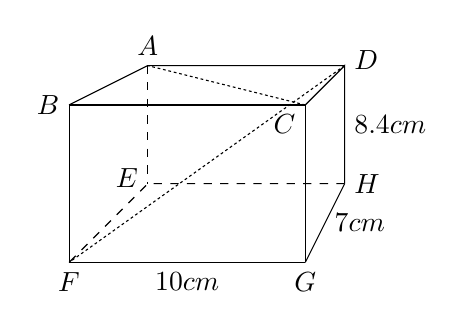
\begin{tikzpicture}
                      \draw (0,0) node [below] {$F$} --(3,0) node [below] {$G$} node[midway, below] {$10cm$};
                      \draw (3,0)--(3.5,1) node [right] {$H$} node [midway, right] {$7cm$};
                      \draw[dashed] (3.5,1)--(1,1) node [above=2pt, left] {$E$} --(0,0);
                      \draw (0,0)--(0,2) node[left] {$B$}--(3,2) node[below left] {$C$} --(3,0);
                      \draw (0,2)--(1,2.5)--(3.5,2.5) node[above=2pt, right] {$D$};
                      \draw (3,2)--(3.5,2.5)--(3.5,1) node [midway, right] {$8.4cm$};
                      \draw[dashed] (1,2.5) node [above] {$A$} --(1,1);
                      \draw[dash pattern=on 1pt off 1pt] (3.5,2.5) -- (0,0);
                      \draw[dash pattern=on 1pt off 1pt] (3,2) -- (1, 2.5);
                  \end{tikzpicture}
              \end{center}
        \item The diagram below shows a cuboid with volume of $400cm^3$, height of $10.5cm$,
              $AD = 2DC$. Find the angle formed by angle $AG$ and plane $ADHE$.
              \begin{center}
                  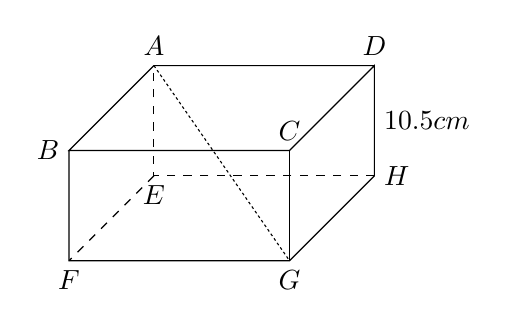
\begin{tikzpicture}[scale=1.4]
                      \draw (2,1,0) node [above] {$D$} --(0,1,0) node [above] {$A$} --(0,1,2) node [left] {$B$} --(2,1,2)node [above] {$C$} --(2,1,0) --(2,0,0) node [right] {$H$} node [midway, right] {$10.5cm$} --(2,0,2) node [below] {$G$} --(0,0,2) node [below] {$F$} --(0,1,2);
                      \draw (2,1,2)--(2,0,2);
                      \draw[dashed](2,0,0)--(0,0,0) node [below] {$E$}--(0,1,0);
                      \draw[dashed](0,0,0)--(0,0,2);
                      \draw[dash pattern=on 1pt off 1pt] (0, 1, 0) -- (2, 0, 2);
                  \end{tikzpicture}
              \end{center}
        \item The diagram below shows a reception room with a square floor with side length
              of $6m$. Given that the elevation angle of corner $C$ measured from corner $A$
              is $30^\circ$, find the angle formed by the line connecting corner $A$ and $B$
              with the floor.
              \begin{center}
                  \includegraphics{reception.png}
              \end{center}
        \item The diagram below shows a cuboid with length of $8cm$, width of $5cm$ and
              height of $6cm$, $M$ is the midpoint of $BF$. Find the angle formed by plane
              $HDM$ and plane $ADHE$.
              \begin{center}
                  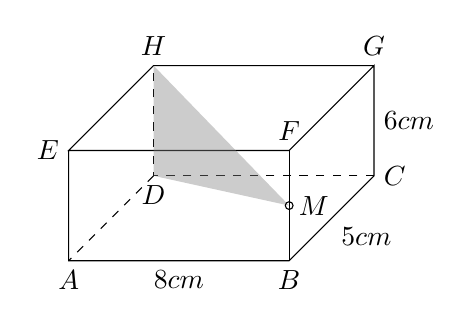
\begin{tikzpicture}[scale=1.4]
                      \draw (2,1,0) node [above] {$G$} --(0,1,0) node [above] {$H$} --(0,1,2) node [left] {$E$} --(2,1,2)node [above] {$F$} --(2,1,0) --(2,0,0) node [right] {$C$} node [midway, right] {$6cm$} --(2,0,2) node [below] {$B$}  node [midway, below right] {$5cm$} --(0,0,2) node [below] {$A$}  node [midway, below] {$8cm$} --(0,1,2);
                      \draw (2,1,2)--(2,0,2);
                      \draw[dashed](2,0,0)--(0,0,0) node [below] {$D$}--(0,1,0);
                      \draw[dashed](0,0,0)--(0,0,2);
                      \fill [color=gray, opacity=0.4] (0, 1, 0) -- (0, 0, 0) -- (2, 0.5, 2) -- cycle;
                      \draw (2, 0.5, 2) circle (1pt) node [right] {$M$};
                  \end{tikzpicture}
              \end{center}
        \item The diagram below shows a pyramid with a square base, its lateral edge $SD$ is
              perpendicular to its base. Given that $BC = 2\sqrt{2}cm$, $SB = 5cm$. Find:
              \begin{enumerate}
                  \item The angle formed by plane $SAD$ and plane $SBD$.
                  \item The angle formed by lateral edge $SA$ and base $ABCD$.
              \end{enumerate}
              \begin{center}
                  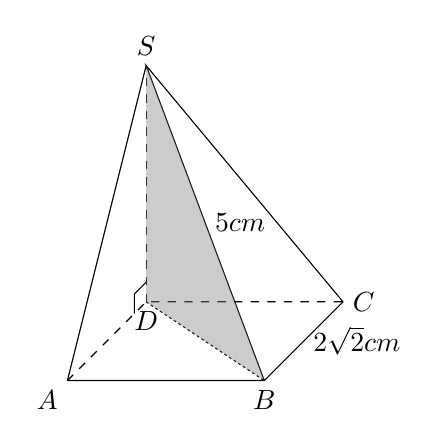
\begin{tikzpicture}
                      \tikzstyle{point}=[circle,thick,draw=black,fill=black,inner sep=0pt,minimum width=4pt,minimum height=4pt]
                      \node (a) at (0,0) {};
                      \node (b) at (2.5,0) {};
                      \node (c) at (3.5,1) {};
                      \node (d) at (1,1) {};
                      \node (e) at (1,4) {};
                      \draw (a.center) node [below left] {$A$} -- (b.center) node [below] {$B$} -- (c.center) node [ right] {$C$} node [midway, right] {$2\sqrt{2}cm$} -- (e.center) node [above] {$S$} -- (b.center) node [midway, right] {$5cm$};
                      \draw (a.center) -- (e.center);
                      \draw[dashed] (a.center) -- (d.center) -- (c.center);
                      \draw[dashed] (d.center) node [below] {$D$} -- (e.center);
                      \draw (1, 1.25) -- (0.85, 1.1) -- (0.85, 0.85);
                      \draw[dash pattern=on 1pt off 1pt] (d.center) -- (b.center);
                      \fill [fill=gray, opacity=0.4] (d.center) -- (b.center) -- (e.center) -- cycle;
                  \end{tikzpicture}
              \end{center}
        \item The diagram below shows a right prism with a rectangular base $ABCD$ with
              length of $28cm$ and width of $20cm$. Assume that plane $VBC$ and the base of
              the pyramid forms a $60^\circ$ angle. Find the angle formed by plane $VAB$ and
              the base.
              \begin{center}
                  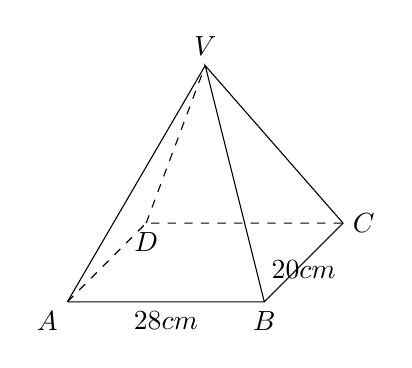
\begin{tikzpicture}
                      \tikzstyle{point}=[circle,thick,draw=black,fill=black,inner sep=0pt,minimum width=4pt,minimum height=4pt]
                      \node (a) at (0,0) {};
                      \node (b) at (2.5,0) {};
                      \node (c) at (3.5,1) {};
                      \node (d) at (1,1) {};
                      \node (e) at (1.75,3) {};
                      \draw (a.center) node [below left] {$A$} -- (b.center) node [below] {$B$} node [midway, below] {$28cm$} -- (c.center) node [ right] {$C$} node [midway, right=12pt, below=-4pt] {$20cm$} -- (e.center) node [above] {$V$} -- (b.center);
                      \draw (a.center) -- (e.center);
                      \draw[dashed] (a.center) -- (d.center) -- (c.center);
                      \draw[dashed] (d.center) node [below] {$D$} -- (e.center);
                  \end{tikzpicture}
              \end{center}
        \item The diagram below shows a regular cuboid with a square base. Given that $VE =
                  \frac{5}{2}AD$. Find:
              \begin{enumerate}
                  \item The angle formed by the angle $VA$ and the base $ABCD$.
                  \item The angle formed by plane $VAD$ and the base.
              \end{enumerate}
              \begin{center}
                  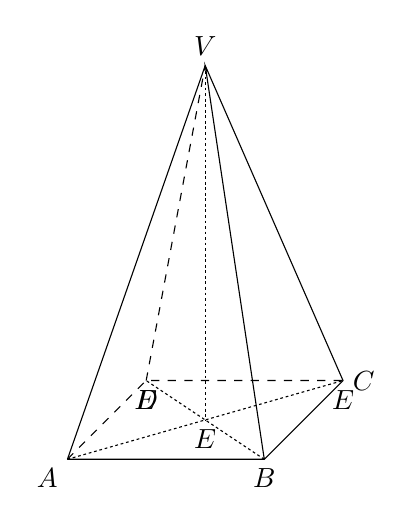
\begin{tikzpicture}
                      \tikzstyle{point}=[circle,thick,draw=black,fill=black,inner sep=0pt,minimum width=4pt,minimum height=4pt]
                      \node (a) at (0,0) {};
                      \node (b) at (2.5,0) {};
                      \node (c) at (3.5,1) {};
                      \node (d) at (1,1) {};
                      \node (e) at (1.75,5) {};
                      \draw (a.center) node [below left] {$A$} -- (b.center) node [below] {$B$} -- (c.center) node [ right] {$C$} -- (e.center) node [above] {$V$} -- (b.center);
                      \draw (a.center) -- (e.center);
                      \draw[dashed] (a.center) -- (d.center) -- (c.center);
                      \draw[dashed] (d.center) node [below] {$D$} -- (e.center);
                      \node (f) at (1.75, 0.5) {};
                      \draw[dash pattern=on 1pt off 1pt] (e.center) -- (f.center) node [below] {$E$};
                      \draw[dash pattern=on 1pt off 1pt] (a.center) -- (c.center) node [below] {$E$};
                      \draw[dash pattern=on 1pt off 1pt] (b.center) -- (d.center) node [below] {$E$};
                  \end{tikzpicture}
              \end{center}
        \item Find the distance from the Panama City$(9^\circ N, 79^\circ 30' W)$ to Toronto
              $(43^\circ 45' N, 79^\circ 30' W)$. (Express your answer in nautical miles)
        \item Tokyo and Adelaide are located at the same longitude, their latitude are
              $35^\circ 45' N$ and $35^\circ S$ respectively. Find the distance between two
              cities along the parallel of latitude.
        \item A plane flies $2000$\emph{NM} along the equator, Find the difference of
              longitude between the point of departure and the destination.
        \item Location $M$ and $N$ are both located at the parallel of latitude $45^\circ$
              north to the equator with a difference in longitude of $20^\circ$. Find the
              distance between $M$ and $N$ along the parallel of latitude. (Express your
              answer in nautical miles)
        \item Location $X$ and $Y$ are on the parallel of latitude $20^\circ$ north to the
              equator, their longitude are $45^\circ E$ and $80^\circ E$ respectively. Find
              the distance between location $X$ and $Y$ along the parallel of latitude.
              (Express your answer in nautical miles)
        \item A plane flies from $A(42^\circ E)$ to $B(20^\circ E)$ along the equator, then
              it flies from $B$ due north to $C(30^\circ N)$. Find the distance the plane
              flies in total.
        \item Assume that $A$ is located $1000$\emph{NM} due north of the equator,
              $600$\emph{NM} due east of the Greenwich Meridian, find the longitude and
              latitude of $A$.
        \item A plane flies from $P(15^\circ N, 30^\circ E)$ $2000$\emph{NM} due south to
              $B$, find the longitude and latitude of $B$. Another plane flies from $P$
              $3000$\emph{NM} due east to $C$, find the longitude and latitude of $C$.
        \item A plane flies from $A(130^\circ E)$ along the equator to $B(120^\circ 30' E)$
              along the equator, then flies from $B$ due north to $C(20^\circ 45')$. Assume
              that the average speed of the plane is $300\text{\emph{NM}}/hr$ throughout the
              journey, find the flight duration for the whole journey.
        \item A plane flies from $A(50^\circ N, 10^\circ E)$ due east to $B(45^\circ E)$.
              \begin{enumerate}
                  \item Find the flight distance of the plane. (Express your answer in nautical miles)
                  \item Assume that the speed of the plane is $420\text{\emph{NM}}/hr$ in average, find
                        the flight duration of the plane.
              \end{enumerate}
        \item Given that three locations $P$, $Q$ and $R$ are located on the same parallel of
              latitude $40^\circ$ north to the equator, The longitude of $P$ and $R$ are
              $10^\circ 30' W$ and $4^\circ 30' E$, $Q$ is located at the middle of $P$ and
              $R$.
              \begin{enumerate}
                  \item Find the difference of longitude between $P$ and $R$.
                  \item Find the longitude of $Q$.
                  \item Find the distance between $P$ and $R$ along the parallel of latitude.
                  \item A ship sails from $P$ to $Q$ along the parallel of latitude with a speed of
                        $18\text{\emph{NM}}/hr$, find the sailing duration of the ship.
              \end{enumerate}
    \end{enumerate}
\end{multicols}
\end{document}